\documentclass[12pt,]{article}
\usepackage{lmodern}
\usepackage{amssymb,amsmath}
\usepackage{ifxetex,ifluatex}
\usepackage{fixltx2e} % provides \textsubscript
\ifnum 0\ifxetex 1\fi\ifluatex 1\fi=0 % if pdftex
  \usepackage[T1]{fontenc}
  \usepackage[utf8]{inputenc}
\else % if luatex or xelatex
  \ifxetex
    \usepackage{mathspec}
  \else
    \usepackage{fontspec}
  \fi
  \defaultfontfeatures{Ligatures=TeX,Scale=MatchLowercase}
\fi
% use upquote if available, for straight quotes in verbatim environments
\IfFileExists{upquote.sty}{\usepackage{upquote}}{}
% use microtype if available
\IfFileExists{microtype.sty}{%
\usepackage{microtype}
\UseMicrotypeSet[protrusion]{basicmath} % disable protrusion for tt fonts
}{}
\usepackage[margin=1in]{geometry}
\usepackage{hyperref}
\hypersetup{unicode=true,
            pdfauthor={Xuan Son Le (4669361), Freie Universität Berlin},
            pdfborder={0 0 0},
            breaklinks=true}
\urlstyle{same}  % don't use monospace font for urls
\usepackage{color}
\usepackage{fancyvrb}
\newcommand{\VerbBar}{|}
\newcommand{\VERB}{\Verb[commandchars=\\\{\}]}
\DefineVerbatimEnvironment{Highlighting}{Verbatim}{commandchars=\\\{\}}
% Add ',fontsize=\small' for more characters per line
\usepackage{framed}
\definecolor{shadecolor}{RGB}{248,248,248}
\newenvironment{Shaded}{\begin{snugshade}}{\end{snugshade}}
\newcommand{\KeywordTok}[1]{\textcolor[rgb]{0.13,0.29,0.53}{\textbf{#1}}}
\newcommand{\DataTypeTok}[1]{\textcolor[rgb]{0.13,0.29,0.53}{#1}}
\newcommand{\DecValTok}[1]{\textcolor[rgb]{0.00,0.00,0.81}{#1}}
\newcommand{\BaseNTok}[1]{\textcolor[rgb]{0.00,0.00,0.81}{#1}}
\newcommand{\FloatTok}[1]{\textcolor[rgb]{0.00,0.00,0.81}{#1}}
\newcommand{\ConstantTok}[1]{\textcolor[rgb]{0.00,0.00,0.00}{#1}}
\newcommand{\CharTok}[1]{\textcolor[rgb]{0.31,0.60,0.02}{#1}}
\newcommand{\SpecialCharTok}[1]{\textcolor[rgb]{0.00,0.00,0.00}{#1}}
\newcommand{\StringTok}[1]{\textcolor[rgb]{0.31,0.60,0.02}{#1}}
\newcommand{\VerbatimStringTok}[1]{\textcolor[rgb]{0.31,0.60,0.02}{#1}}
\newcommand{\SpecialStringTok}[1]{\textcolor[rgb]{0.31,0.60,0.02}{#1}}
\newcommand{\ImportTok}[1]{#1}
\newcommand{\CommentTok}[1]{\textcolor[rgb]{0.56,0.35,0.01}{\textit{#1}}}
\newcommand{\DocumentationTok}[1]{\textcolor[rgb]{0.56,0.35,0.01}{\textbf{\textit{#1}}}}
\newcommand{\AnnotationTok}[1]{\textcolor[rgb]{0.56,0.35,0.01}{\textbf{\textit{#1}}}}
\newcommand{\CommentVarTok}[1]{\textcolor[rgb]{0.56,0.35,0.01}{\textbf{\textit{#1}}}}
\newcommand{\OtherTok}[1]{\textcolor[rgb]{0.56,0.35,0.01}{#1}}
\newcommand{\FunctionTok}[1]{\textcolor[rgb]{0.00,0.00,0.00}{#1}}
\newcommand{\VariableTok}[1]{\textcolor[rgb]{0.00,0.00,0.00}{#1}}
\newcommand{\ControlFlowTok}[1]{\textcolor[rgb]{0.13,0.29,0.53}{\textbf{#1}}}
\newcommand{\OperatorTok}[1]{\textcolor[rgb]{0.81,0.36,0.00}{\textbf{#1}}}
\newcommand{\BuiltInTok}[1]{#1}
\newcommand{\ExtensionTok}[1]{#1}
\newcommand{\PreprocessorTok}[1]{\textcolor[rgb]{0.56,0.35,0.01}{\textit{#1}}}
\newcommand{\AttributeTok}[1]{\textcolor[rgb]{0.77,0.63,0.00}{#1}}
\newcommand{\RegionMarkerTok}[1]{#1}
\newcommand{\InformationTok}[1]{\textcolor[rgb]{0.56,0.35,0.01}{\textbf{\textit{#1}}}}
\newcommand{\WarningTok}[1]{\textcolor[rgb]{0.56,0.35,0.01}{\textbf{\textit{#1}}}}
\newcommand{\AlertTok}[1]{\textcolor[rgb]{0.94,0.16,0.16}{#1}}
\newcommand{\ErrorTok}[1]{\textcolor[rgb]{0.64,0.00,0.00}{\textbf{#1}}}
\newcommand{\NormalTok}[1]{#1}
\usepackage{graphicx,grffile}
\makeatletter
\def\maxwidth{\ifdim\Gin@nat@width>\linewidth\linewidth\else\Gin@nat@width\fi}
\def\maxheight{\ifdim\Gin@nat@height>\textheight\textheight\else\Gin@nat@height\fi}
\makeatother
% Scale images if necessary, so that they will not overflow the page
% margins by default, and it is still possible to overwrite the defaults
% using explicit options in \includegraphics[width, height, ...]{}
\setkeys{Gin}{width=\maxwidth,height=\maxheight,keepaspectratio}
\IfFileExists{parskip.sty}{%
\usepackage{parskip}
}{% else
\setlength{\parindent}{0pt}
\setlength{\parskip}{6pt plus 2pt minus 1pt}
}
\setlength{\emergencystretch}{3em}  % prevent overfull lines
\providecommand{\tightlist}{%
  \setlength{\itemsep}{0pt}\setlength{\parskip}{0pt}}
\setcounter{secnumdepth}{5}
% Redefines (sub)paragraphs to behave more like sections
\ifx\paragraph\undefined\else
\let\oldparagraph\paragraph
\renewcommand{\paragraph}[1]{\oldparagraph{#1}\mbox{}}
\fi
\ifx\subparagraph\undefined\else
\let\oldsubparagraph\subparagraph
\renewcommand{\subparagraph}[1]{\oldsubparagraph{#1}\mbox{}}
\fi

%%% Use protect on footnotes to avoid problems with footnotes in titles
\let\rmarkdownfootnote\footnote%
\def\footnote{\protect\rmarkdownfootnote}

%%% Change title format to be more compact
\usepackage{titling}

% Create subtitle command for use in maketitle
\newcommand{\subtitle}[1]{
  \posttitle{
    \begin{center}\large#1\end{center}
    }
}

\setlength{\droptitle}{-2em}
  \title{\textbf{Logistische Regression}}
  \pretitle{\vspace{\droptitle}\centering\huge}
  \posttitle{\par}
  \author{Xuan Son Le (4669361), Freie Universität Berlin}
  \preauthor{\centering\large\emph}
  \postauthor{\par}
  \predate{\centering\large\emph}
  \postdate{\par}
  \date{02/04/2018}

\usepackage{caption}
\captionsetup[figure]{name=Abbildung}

\begin{document}
\maketitle

\begin{center}\rule{0.5\linewidth}{\linethickness}\end{center}

\textbf{Abstract}: Im Rahmen der Abschlussarbeit des Moduls
Programmieren mit R im Wintersemester 2017/2018 an der Freie Universität
Berlin wird für diese Arbeit die statistische Methode namens binäres
Logit-Modell ausgewählt. Diese Arbeit besteht aus zwei großen
Hauptteilen: der Theorieteil, wobei die ausgewählte Methode theoretisch
vorgestellt wird und der Implementierungsteil, welcher die Erklärung der
Funktionalität vom selbst entwickelten Paket beinhaltet. Im Theorieteil
wird zunächst ein Überblick über die grundliegende Funktionsweise vom
(binären) Logit-Modell widergegeben. Die Grundidee von Generalisierten
linearen Modellen wird anschließend kurz eingeführt, bevor der Aufbau
vom binären Logit-Modell durch das Maximum Likelihood Verfahren
vorgenommen wird. Demzufolge folgt die Interpretation der Koeffizienten
vom binären Logit-Modell. Schließlich werden im Implementierungsteil
alle Funktionen vom R-Paket schritterweise vorgestellt.

\textbf{Keywords:} \emph{Logit-Modell, logistische Regression, Paket, R}

\begin{center}\rule{0.5\linewidth}{\linethickness}\end{center}

\newpage

\section{Motivation}\label{motivation}

Die Anwendung von der klassischen linearen Regression ist für binäre
(binomiale oder dichotome) Zielvariable (Response- oder zu erklärende
Variable), welche lediglich zwei Werte (ja/nein, mänlich/weiblich,
erfolgreich/nicht erfolgreich, etc.) annehmen kann, nicht mehr geeignet,
da die Zielvariable von der linearen Regression metrisch skaliert ist.
Oft wird binäre Variable als 0/1-Variable kodiert, das heißt sie nimmt
nur den Wert 0 oder 1 an. Die folgende Grafik stellt den Ansatz
graphisch dar, binäre Variable durch lineare Regression zu modellieren:

\begin{figure}[h]

{\centering 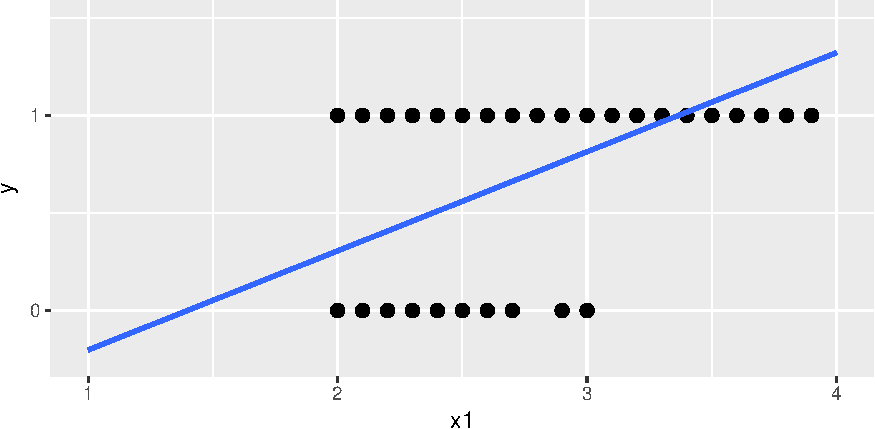
\includegraphics{logisticRegression_files/figure-latex/unnamed-chunk-1-1} 

}

\caption{Beispielshafte lineare Regression für binäre Zielvariable}\label{fig:unnamed-chunk-1}
\end{figure}

Graphisch lässt sich festlegen, dass die lineare Regression den
Wertebereich {[}0,1{]} von binären Responsevariablen sehr schnell
verlässt. Aus diesem Grund wird ein ganz anderer Ansatz benötigt, um
binäre Zielvariable zu modellieren, nämlich das binäre Logit-Modell
(auch binäre logistische Regression oder binäres logistisches
Regressionsmodell). In der Statistik lassen sich Logit-Modelle noch in
multinomiale und kumulative Logit-Modelle aufteilen, je nachdem ob die
abhängige Variable multinominal- oder ordinalskaliert sind . Diese
Arbeit beschäftigt sich mit dem binären Logit-Modell, welches den
Zusammenhang zwischen einer binären abhängigen Variable und
einer/mehreren unabhängigen Variablen untersucht. Bei allen Arten von
Logit-Modellen können die unabhängigen Variablen (erklärende oder
Kovariablen) beliebig skaliert sein.

Im Unterschied zu der klassischen linearen Regression, welche den wahren
Wert einer Zielvariable vorhersagt, interessiert sich das binäre
Logit-Modell eher für die Wahrscheinlichkeit, dass die Zielvariable den
Wert 1 annimmt. Das Hauptziel vom binären Logit-Modell ist es, die
Wahrscheinlichkeit für den Eintritt der Zielvariable vorherzusagen.
Dadurch soll die folgende theoretische Fragestellung beantwortet werden:
\emph{Wie stark ist der Einfluss von den unabhängigen (erklärenden)
Variablen auf die Wahrscheinlichkeit, dass die abhängige (zu erklärende
/ Response) Variable eintritt beziehungsweise den Wert 1 annimmt?} In
der Praxis kann diese Fragestellung beispielsweise so formuliert werden:
``Haben Alter, Geschlecht, Berufe oder andere Merkmale der Kunden
Einfluss auf die Wahrscheinlichkeit, dass sie ein Kredit rechtzeitig
zurückzahlen?'' oder ``Lässt sich die Wahrscheinlichkeit, dass es
regnet, durch die Temparatur, die Windstärke oder
Sonnenstrahlungsintensität vorhersagen?''.

\section{Das binäre Logit-Modell}\label{das-binare-logit-modell}

Das Logit-Modell ist eine Methode aus der Algorithmenklasse namens
\emph{Generalisierte Lineare Modelle} (engl. generalized linear model,
kurz GLM), welche eine Verallgemeinerung des klassischen linearen
Regressionsmodells anstrebt. Dazu gehören noch die klassische lineare
Regression, Probitmodell und Poisson-Regression. Die Grundidee von GLM
ist die Transformation der linearen Regressionsgleichung, so dass der
Wertebereich der vorhergesagten Zielvariable dem gewünschten entspricht.
Die Theorie von GLMs wurde von Nelder und Wedderburn entwickelt. In
Anlehnung an Schlittgen, R. (2013) können Modelle zu GLMs zugeordnet
werden, wenn sie: 1. 2.

\newpage 

\subsection{Modellspezifikation}\label{modellspezifikation}

Die folgende Modellspezifikation basiert sich auf Kapitel 9.1 aus dem
Buch \emph{Regressionsanalysen mit R} (Schlittgen
\protect\hyperlink{ref-schlittgen2013regressionsanalysen}{2013},
S.215-225).

Gegeben seien n unabhängige Beobachtungen \(y_1, y_2, ...,y_n\) der
binären Zielvariable \(\mathbf{Y}\). Ein Verteilungsmodell für
\(\mathbf{Y}\) ist die Binomialverteilung:
\(\mathbf{Y}_i \sim B(1, \pi_i)\) mit \(\pi_i = P(Y_i = 1)\). Für diese
Arbeit wird \(\pi_i = (\pi_1, \pi_2, ..., \pi_n)\) als die
Eintrittwahrscheinlichkeit von der einzelnen \(\mathbf{Y}_i\) benannt.
Weiterhin seien p erklärende Variablen
\(\mathbf{X}_0,\mathbf{X}_1,..,\mathbf{X}_p\) gegeben mit jeweils n
unabhängigen Beobachtungen
\(\mathbf{X}_j = (x_{1j}, x_{2j},..., x_{nj})\) - j \(\in\)
\{0,1,2,..,p\} - gegeben. Daraus ergeben sich p Koeffizienten
\(\beta = (\beta_0, \beta_1, \beta_2,..., \beta_p)\), welche die Stärke
den Zusammenhang zwischen die einzelne erklärende Variable mit der
Zielvariable widerspiegeln. Dabei ist es sinnvoll, diese in einer
Designmatrix \(\mathbf{X}\) zu speichern. Da der Interzept (\(\beta_0\))
ebenfalls geschätzt werden soll, sind alle Werte der ersten Spalte von X
gleich Eins, also \(x_{10} = x_{20} = ... = x_{n0} = 1\).
Zusammengefasst lässt sich die Designmatrix wie folgt darstellen: \[
\mathbf{X} =
 \begin{pmatrix}
    1 & x_{11} & x_{12} & \cdots & x_{1p} \\
    1 & x_{21} & x_{22} & \cdots & x_{2p} \\
    1 & x_{31} & x_{32} & \cdots & x_{3p} \\
    \vdots  & \vdots  & \vdots & \ddots & \vdots \\
    1 & x_{n1} & x_{n2} & \cdots & x_{np}
 \end{pmatrix}
\] Die dazugehörige lineare Regressionsgleichung lautet:
\(\mathbf{Y} = \mathbf{X}.\beta + \epsilon\) mit
\(\epsilon = (\epsilon_1, \epsilon_2, \epsilon_3, ..., \epsilon_n)\) als
die Abweichung der einzelnen Schätzungen gegenüber dem wahren Wert,
wobei \(\mathbf{Y}\) ein (nx1)-Vektor, \(\mathbf{X}\) ein (nxp) und
\(\beta_i\) sowie \(\epsilon_i\) ein (px1)-Vektor ist.

Die einzelne Beobachtung lässt sich wie folgt darstellen: \[
y_i = \beta_0 + \beta_1.x_{i1} + \beta_2.x_{i2} + ... + \beta_p.x_{ip} + \epsilon_i = \mathbf{x'}_i.\beta + \epsilon_i \qquad \forall_i = 1,2,3,...,n
\]

Wobei \(\mathbf{x}_i\) der i-ten Zeile der Designmatrix \(\mathbf{X}\)
entspricht. Da bei der Multiplikation A.B die Regel gilt, dass die
Spaltenanzahl von A der Zeilenanzahl von B entsprechen muss. Da
\(\beta\) ein (px1)-Vektor ist, muss \(\mathbf{x}_i\) (px1-Vektor) in
\(\mathbf{x'}_i\) (1xp-Vektor) transponiert werden, damit die
Multiplikation durchführbar ist.

Um die Werte im Bereich der reellen Zahlen von der linearen Regression
auf dem Wertebereich von Wahrscheinlichkeiten zwischen 0 und 1 zu
beschränken, sollte die rechte Seite der Gleichung transformiert werden.
Das Ziel ist es, eine sinnvolle Verteilungsfunktion (Responsefunktion)
zu finden, deren Wertebereich in {[}0,1{]} liegt:
\(\pi_i = P(\mathbf{Y_i} = 1) = F(\beta_0 + \beta_1.x_{i2} + \beta_2.x_{i3} + ... + \beta_p.x_{ip}) = F(\eta_i)\).
Der lineare Prädikator
\(\eta_i = \beta_0 + \beta_1.x_{i2} + \beta_2.x_{i3} + ... + \beta_p.x_{ip} = \mathbf{x'}_i.\beta \ \ (1)\)
wird ebenfalls als Linkfunktion genannt, weil dadurch eine Verbindung
(Link) zwischen der Eintrittwahrscheinlichkeit und den unabhängigen
Variablen erfolgt wird. Für das binäre Logit-Modell wird anstelle der
Responsefunktion die standardisierte logistische Verteilung verwendet:

\[
F(\eta_i) = Logist(\eta_i) = \frac{\exp(\eta_i)}{1 + \exp(\eta_i)} \quad (2)
\] Da durch die Responsefunktion die Eintrittwahrscheinlichkeit
\(\pi_i\) modelliert werden soll, ergibt sich die Gleichung für das
binäre Logit-Modell wie folgt:

\[
\pi_i = \frac{\exp(\eta_i)}{1 + \exp(\eta_i)} = \frac{\exp(\beta_0 + \beta_1.x_{i2} + \beta_2.x_{i3} + ... + \beta_p.x_{ip})}{1 + \exp(\beta_0 + \beta_1.x_{i2} + \beta_2.x_{i3} + ... + \beta_p.x_{ip})} = \frac{\exp(\mathbf{x'}_i.\beta)}{1+\exp(\mathbf{x'}_i.\beta)} \quad (3)
\] Dabei kann \(\pi_i\) maximal den Wert 1 nehmen, wenn \(\exp(\eta_i)\)
sehr groß ist und minimal den Wert 0, wenn \(\exp(\eta_i)\) sehr nah
rechts von 0 liegt. \(\exp(\eta_i)\) kann nicht negativ sein. Diese
Gleichung erfüllt somit die Anforderung bezüglich dem Wertebereich von
Wahrscheinlichkeiten.

Soll die Gleichung nach dem linearen Prädikator \(\eta_i\) gelöst
werden, ergibt sich schließlich die Logit-Linkfunktion: \[
\begin{aligned}
\pi_i.(1 + \exp(\eta_i)) &= \exp(\eta_i) \\
\Leftrightarrow \pi_i + \pi_i.\exp(\eta_i) &= \exp(\eta_i) \\
\Leftrightarrow \pi_i &= \exp(\eta_i) - \pi_i.\exp(\eta_i)  \\
\Leftrightarrow \pi_i &= \exp(\eta_i).(1-\pi_i) \\
\Leftrightarrow \exp(\eta_i) &= \frac{\pi_i}{1-\pi_i} \\
\Leftrightarrow \eta_i &= \ln(\frac{\pi_i}{1-\pi_i}) \quad (4)\\
\end{aligned} 
\]

Es gilt nämlich: \[
\beta_0 + \beta_1.x_{i2} + \beta_2.x_{i3} + ... + \beta_p.x_{ip} = \ln(\frac{\pi_i}{1-\pi_i}) \quad (5)
\]

\subsection{Maximum Likelihood
Schätzung}\label{maximum-likelihood-schatzung}

Ähnlich wie bei der linearen Regression muss bei dem binären
Logit-Modell die unbekannten Parameter \(\beta_i\) (i =
0,1,2,\ldots{},k) ebenfalls geschätzt werden. Bei der klassischen
linearen Regression wird die Methode der Kleinsten Quadrate (engl.
\emph{method of least squares}, kurz KQ-Methode) genutzt, um eine
Regressionslinie zu bestimmen, welche die Summe der quadratischen
Abweichungen von den beobachteten Punkten minimiert. Da bei dem binären
Logit-Modell nicht der wahre Wert der Zielvariable sondern die
Eintrittswahrscheinlichkeit geschätzt wird, ist die Abweichung zwischen
dem wahren Wert und dem geschätzten Wert nicht mehr aussagekräftig wie
bei der linearen Regression. Die Koeffizienten müssen anders geschätzt
werden. Dementsprechend wird bei dem binären Logit-Modell die sogenannte
Maximum Likelihood Schätzung (kurz ML-Schätzung) eingesetzt. Abbildung
.. zeigt ein Beispiel mit zwei mögliche binäre logistiche
Regressionskurven, die durch das Maximum Likelihood optimiert werden
sollen. Es gibt unendlich viele solche Kurven. Das Ziel ist es, die
Kurve mit dem höchsten Maximum Likelihood herauszufinden.

\begin{figure}[h]

{\centering 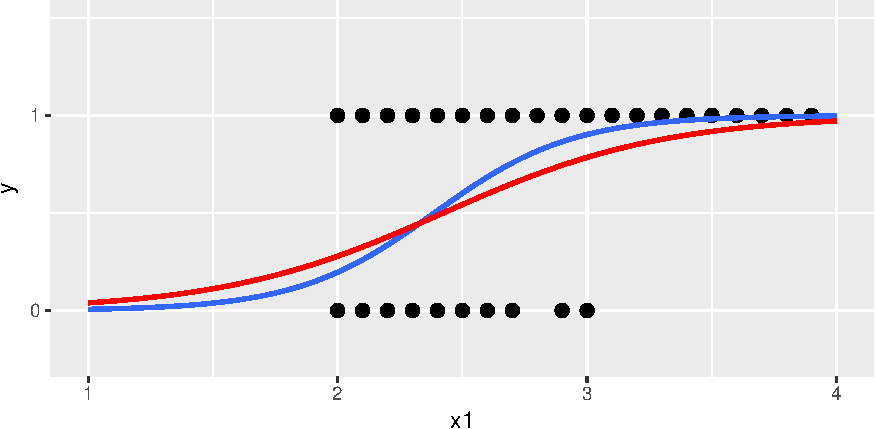
\includegraphics{logisticRegression_files/figure-latex/unnamed-chunk-2-1} 

}

\caption{Beispielshafte logistische Regressionskurve}\label{fig:unnamed-chunk-2}
\end{figure}

Das Ziel der ML-Schätzung besteht darin, die Eintrittswahrscheinlichkeit
für die empirischen Beobachtungswerte zu maximieren. Dafür kommt die
(Log-)Likelihood-Funktion zum Einsatz. Im Folgenden wird die
Vorgehensweise zum Lösen der ML-Schätzung anhand der
Log-Likelihood-Funktion wiedergegeben: 1. Maximum Likelihood Funktion 2.
Log-Likelihood-Funktion 3. Score-Funktion (erste Ableitung) 4. Hesse
Matrix (zweite Ableitung) 5. Newton-Raphson-Methode

\subsubsection{Maximum Likelihood
Funktion}\label{maximum-likelihood-funktion}

Gegeben sei \(y_i = 1\) mit der Eintrittswahrscheinlichkeit \(\pi_i\),
und \(y_i = 0\) mit der Gegenwahrscheinlichkeit \((1-\pi_i)\). Die
Likelihood-Funktion lässt sich wie folgt definieren: \[
\mathcal{L}(\beta) = {\prod_{i=1}^{n} \pi_i^{y_i}.(1-\pi_i)^{1-y_i}} \quad (6)
\] Wenn \(y_i\) gleich 1 ist, ergibt sich für die betroffene Beobachtung
die Eintrittswahrscheinlichkeit \(\pi_i\) und umgekehrt. Das Likelihood
ist gleich die Multiplikation der Wahrscheinlichkeiten von allen
Beobachtungen. Dieses soll maximiert werden.

Da \(\pi_i\) von dem linearen Prädikator \(\eta_i\) abhängt, ist die
Likelihood-Funktion von \(\beta\) abhängig. Wird
\(\pi_i = \frac{\exp(\eta_i)}{1 + \exp(\eta_i)}\) in die
Likelihood-Funktion eingesetzt, ergibt sich:

\[
\mathcal{L}(\beta) = {\prod_{i=1}^{n} \Bigg[ \Big( \frac{\exp(\eta_i)}{1 + \exp(\eta_i)} \Big)^{y_i}.\Big(1-\frac{\exp(\eta_i)}{1 + \exp(\eta_i)}\Big)^{1-y_i}}\Bigg] \quad (7)
\]

\subsubsection{Log-Likelihood-Funktion}\label{log-likelihood-funktion}

Der Versuch, Gleichung (7) zu differenzieren und nach \(\beta\) zu
lösen, um die Extremwerte zu finden, ist extrem aufwendig, weil sie eine
Serie von Multiplikationen enthält. Wegen den exponentialen Komponenten
kann die logistische Funktion aus der Mathematik zur Vereinfachung der
Likelihood-Funktion Einsatz finden. Da die logistische Funktion eine
monotone Funktion ist, entspricht jedes Maximum von der
Likelihood-Funktion dem Maximum von der Log-Likelihood-Funktion und
umgekehrt. Es gelgen für den Logarithmus folgende Regelungen (seien alle
Vorzeichenvoraussetzungen für den Logarithmus erfüllt): \[
\begin{aligned}
(8) \quad &\ln(\prod_{i=1}^{n}x_i) = \ln(x_1.x_2...x_n) = \ln(x_1) + \ln(x_2) + \ ... \ + \ln(x_n) = \sum_{i=1}^{n} \ln(x_i) \\
(9) \quad &\ln(x^\alpha) = \alpha.\ln(x) \\
(10) \quad &\ln(\frac{x}{y}) = \ln(x) - \ln(y)
\end{aligned} 
\]

Dementsprechend lässt die Likelihood-Funktion wie folgt
logarithmisieren: \[
\begin{aligned}
\ell(\beta) = \ln(\mathcal{L}(\beta)) = \quad &\ln \Bigg( \prod_{i=1}^{n} \pi_i^{y_i}.(1-\pi_i)^{1-y_i} \Bigg) \\
\mathrel{\overset{(8)}{=}} \quad &\sum_{i = 1}^{n} \ln \Big(\pi_i^{y_i}.(1-\pi_i)^{1-y_i}\Big) \\
\mathrel{\overset{(9)}{=}} \quad &\sum_{i = 1}^{n} \Big( y_i.\ln(\pi_i) + (1-y_i).\ln(1-\pi_i) \Big) \\
= \quad &\sum_{i = 1}^{n} \Big( y_i.\ln(\pi_i) - y_i.\ln(1-\pi_i) + \ln(1-\pi_i) \Big) \\
\mathrel{\overset{(10)}{=}} \quad &\sum_{i = 1}^{n} \Bigg( y_i.\ln \Big(\frac{\pi_i}{1-\pi_i}\Big) + \ln(1-\pi_i) \Bigg) \\
\mathrel{\overset{(4),(3)}{=}} \ &\sum_{i = 1}^{n} \Bigg( y_i.\eta_i + \ln \Big( 1- \frac{\exp(\eta_i)}{1 + \exp(\eta_i)} \Big) \Bigg) \\
= \quad &\sum_{i = 1}^{n} \Bigg( y_i.\eta_i + \ln \Big( \frac{1}{1+\exp(\eta_i)}\Big) \Bigg) \\
= \quad &\sum_{i = 1}^{n} \Big( y_i.\eta_i - \ln (1 + exp(\eta_i)) \Big) \quad (11)
\end{aligned}
\]

\subsubsection{Score-Funktion}\label{score-funktion}

Zum Herausfinden des ML-Schätzers, welcher die log-Likelihood-Funktion
optimiert, wird Gleichung (10) nach \(\beta\) differenziert. Die erste
Ableitung von der log-Likelihood-Funktion wird als Score-Funktion
benannt:

\[
\begin{aligned}
s(\beta) = \frac{\partial}{\partial \beta}  \ell(\beta) &= \frac{\partial}{\partial \beta} \sum_{i = 1}^{n} \Big( y_i.\eta_i - \ln (1 + \exp(\eta_i)) \Big) \quad \\
&\mathrel{\overset{(1)}{=}} \frac{\partial}{\partial \beta} \sum_{i = 1}^{n} \Big( y_i.\mathbf{x'}_i.\beta  - \ln (1 + \exp(\mathbf{x'}_i.\beta )) \Big) \quad \\ 
\end{aligned}
\]

Seien alle Vorzeichnenanforderungen erfüllt, gelten folgende Regelungen
bezüglich der Differenzierungsrechnung: \[
\begin{aligned}
&(12) \frac{\partial}{\partial t} a.f(t) = (a.f(t))' = a.f'(t) \\
&(13) \frac{\partial}{\partial t} \ln(f(t)) = [\ln(f(t))]' = \frac{f'(t)}{f(t)} \\ 
&(14) \frac{\partial}{\partial t} \exp(f(t)) = [\exp(f(t))]' = f'(t).\exp(f(t)) \\
\end{aligned}
\]

Eingesetzt in die Score-Funktion: \[
\begin{aligned}
s(\beta) &= \sum_{i = 1}^{n} \Bigg( y_i.\mathbf{x'}_i - \frac{\mathbf{x'}_i.\exp(\mathbf{x'}_i.\beta)}{1 + \exp(\mathbf{x'}_i.\beta)} \Bigg) \\
&\mathrel{\overset{(1)}{=}}\sum_{i = 1}^{n} \Bigg[ \mathbf{x'}_i \Bigg( y_i - \frac{\exp(\eta_i)}{1 + \exp(\eta_i)} \Bigg) \Bigg] \\
&\mathrel{\overset{(2)}{=}}  \sum_{i = 1}^{n} \ \mathbf{x'}_i ( y_i - \pi_i) \quad  \\
&= \mathbf{X}'.(y-\pi) \quad (15) 
\end{aligned}
\]

\subsubsection{Hesse Matrix}\label{hesse-matrix}

Da \(s(\beta)\) wegen exponentiellen Komponenten nicht linear von
\(\beta\) abhängt, wird zur Maximierung der Funktion ein iteratives
Verfahren verwendet. Für diese Arbeit wird die Newton-Raphson-Methode
(vgl. \ldots{}) ausgewählt. Dafür muss die zweite Ableitung der Funktion
noch gebildet werden, welche als Hesse-Matrix (H) bezeichnet wird:

\[
\begin{aligned}
\frac{\partial^2}{\partial \beta^2} \ell(\beta) = \frac{\partial}{\partial \beta} s(\beta) = H(\beta) &\mathrel{\overset{(15)}{=}} \frac{\partial}{\partial \beta} \sum_{i = 1}^{n} \ (\mathbf{x'}_i.y_i - \mathbf{x'}_i.\pi_i) \\
&= - \sum_{i = 1}^{n} \Bigg( \mathbf{x'}_i \ .  \Big(\frac{\partial}{\partial \beta} \pi_i \Big) \Bigg) \\
&\mathrel{\overset{(3)}{=}} - \sum_{i = 1}^{n} \Bigg( \mathbf{x'}_i \ .  \Big(\frac{\partial}{\partial \beta} \frac{\exp(\mathbf{x'}_i.\beta)}{1+\exp(\mathbf{x'}_i.\beta)} \Big) \Bigg) \\
\end{aligned}
\]

Wegen \[
\frac{\partial}{\partial t} \frac{f(t)}{g(t)} = \frac{f'(t).g(t) - g'(t).f(t)}{(g(t))^2}
\]

gilt:

\[
\begin{aligned}
\frac{\partial}{\partial \beta} s(\beta) = H(\beta) &= - \sum_{i = 1}^{n} \Bigg[ \mathbf{x'}_i \ . \Bigg( \frac{\mathbf{x'}_i.\exp(\mathbf{x'}_i.\beta).(1+\exp(\mathbf{x'}_i.\beta))-\mathbf{x'}_i.\exp(\mathbf{x'}_i.\beta).\exp(\mathbf{x'}_i.\beta)}{(1+\exp(\mathbf{x'}_i.\beta))^2} \Bigg) \Bigg] \\
&= - \sum_{i = 1}^{n} \Bigg[ \mathbf{x'}_i \ . \frac{\mathbf{x'}_i.\exp(\mathbf{x'}_i.\beta)}{(1+\exp(\mathbf{x'}_i.\beta))^2}  \Bigg] \\
&= - \sum_{i = 1}^{n} \Bigg( \mathbf{x'}_i \ . \frac{\mathbf{x'}_i}{1+\exp(\mathbf{x'}_i.\beta)} . \frac{\exp(\mathbf{x'}_i.\beta)}{1+\exp(\mathbf{x'}_i.\beta)} \Bigg) \\
&\mathrel{\overset{(3)}{=}} - \sum_{i = 1}^{n} \Big( \mathbf{x'}_i . \mathbf{x'}_i . (1-\pi_i) . \pi_i \Big) \\
&= - \sum_{i = 1}^{n} \Big( (\mathbf{x'}_i)^2 . (1-\pi_i) . \pi_i \Big) \\
&= - \sum_{i = 1}^{n} \Big( \mathbf{x'}_i.\mathbf{x}_i . (1-\pi_i) . \pi_i \Big) \quad \\
\end{aligned}
\]

Sei M eine nxn-Matrix mit dem i-ten diagonalen Element
\(\mathbf{M}_{ii} = \pi_i.(1-\pi_i)\) mit \(i \in (1,2,...,n)\), ergibt
sich: \[
s'(\beta) = H(\beta) = - \sum_{i = 1}^{n} \mathbf{x'}_i.\mathbf{x}_i . \mathbf{M}_{ii} = - \mathbf{X}'\mathbf{M}\mathbf{X} \quad (16)
\]

\subsubsection{Newton-Raphson-Methode}\label{newton-raphson-methode}

Die Newton-Raphson-Methode setzt sich zum Ziel, eine nichtlinear lösbare
Funktion zu optimieren. Diese Methode wurde \ldots{} (QUELLE).

Sei \(\mathbf{f}\) eine Funktion von x, \(\mathbf{f'}(x)\) die erste
Ableitung und \(x_0\) die Initiallösung. Das Ziel ist es, die Gleichung
\(\mathbf{f}(x) = 0\) zu lösen. Seien alle Anforderungen der
Differentialrechnung erfüllt, kann eine Verbesserung von \(x_0\) wie
folgt berechnet werden: \[
x_1 = x_0 - \frac{\mathbf{f}(x_0)}{\mathbf{f'}(x_0)}
\]

Wobei eine Verbesserung bedeutet, dass \(\mathbf{f}(x_1)\) näher an 0
liegt als \(\mathbf{f}(x_0)\). Dieser Prozess wird so oft wiederholt,
bis eine akzeptable Lösung anhand der vordefinierten Abbruchskriterien
bestimmt wird: \[
x_{n+1} = x_n - \frac{\mathbf{f}(x_n)}{\mathbf{f'}(x_n)} \quad (17)
\]

\(\mathbf{f}(x)\) repräsentiert für diese Arbeit die Score-Funktion
\(s(\beta)\), da die Gleichung \(s(\beta) = 0\) gelöst werden soll.
Eingesetzt in Gleichung 17 ergibt sich: \[
\begin{aligned}
\beta_{n+1}\quad  = \qquad &\beta_n - \frac{s(\beta)}{s'(\beta)} \\
\mathrel{\overset{(15),(16)}{=}} \quad &\beta_n - \frac{\ \  \mathbf{X}'.(y-\pi)}{- \mathbf{X}'\mathbf{M}\mathbf{X}} \\ \\
= \qquad &\beta_n + (\mathbf{X}'\mathbf{M}\mathbf{X})^{-1}.\mathbf{X}'.(y-\pi) \quad (17)
\end{aligned} 
\]

In Anlehnung an (Quinn \protect\hyperlink{ref-quinn2001newton}{2001})
wird demnächst die Newton-Raphson-Methode anhand einem Pseudocode näher
erläutert: \[
\begin{aligned}
&1 \quad \mathbf{function}(X, y): \\
&2 \qquad \quad   \mathbf{initialisiere} \ \ \beta_0,\ maxIteration,\ i,\ tolerance,\ diff,\ M \\
&3 \qquad \quad  \mathbf{while} \ (diff > tolerance) \\
&4 \qquad \qquad \quad betaChange = (\mathbf{X}'\mathbf{M}\mathbf{X})^{-1}.\mathbf{X}'.(y-\pi) \\
&5 \qquad \qquad \quad diff = | betaChange| \\
&6 \qquad \qquad \quad      i = i + 1 \\
&7 \qquad \qquad \quad      \mathbf{if} \ (i > maxIteration): \\
&8  \qquad \qquad \qquad \qquad          break \\ 
&9 \quad \bf{end} 
\end{aligned}
\]

Es wird eine zulässige Startlösung \(\beta_0\) initialisiert. Je näher
\(s(\beta_0)\) an 0 liegt, umso schneller sollte die Laufzeit der
Schleife sein. Dieses wird bei der Implementierung berücksichtigt, um
herauszufinden, ob es sich lohnt, eine gute Startlösung festzustellen.

\emph{tolerance} ist in der Regel sehr klein positiv und dient als
Indikator für die Konvergenz des Algorithmus. Grundsätzlich sollte die
Differenz \emph{diff} = \(|\beta_{i+1} - \beta_i|\) nach jeder Iteration
immer kleiner werden. Wenn der Algorithmus konvergiert, wird nach einer
bestimmten Anzahl an Iterationen diese Differenz kleiner als der
vorgegebene Konvergenzwert. Wenn die Differenz immer größer als der
Konvergenzwert bleibt, kann festgestellt werden, dass der Algorithmus
nicht konvergiert. Wenn es der Fall ist, terminiert der Algorithmus bei
Erreichung der maximalen Anzahl an Iterationen (\emph{maxIteration}).

\subsection{Intepretation der
Koeffizienten}\label{intepretation-der-koeffizienten}

Im Unterschied zu der linearen Regression lassen sich bei dem binären
Logit-Modell die Koeffizienten nicht direkt interpretieren, da die
Eintrittswahrscheinlichkeit von \(\beta\) durch eine komplexe Funktion
abhängig ist (siehe Gleichung 3). Die Bruchrechnung
\(\frac{\pi_i}{1-\pi_i}\) (Gleichung 4) spielt bei dem binären
Logit-Modell eine besondere Rolle, weil sie der Verbindung zwischen der
Eintrittswahrscheinlichkeit und der Gegenwahrscheinlichkeit direkt
widerspiegelt. Dieses wird als \textbf{Odds} bezeichnet. Der Begriff
\textbf{Chance} ist eine andere Möglichkeit, die \textbf{Odds}
darzustellen. Beispielsweise wird beim Münzwurf von einer 1:1-Chance für
Kopf bespochen, da die Wahrscheinlichkeiten von Kopf und Zahl gleich 0.5
sind und der Odd somit 1 ist. \textbf{Odds} lassen sich wie folgt
zerlegen: \[
\begin{aligned}
Odd(\pi_i) = \frac{P(Y = 1)}{P(Y=0)} = \frac{\pi_i}{1-\pi_i} &\mathrel{\overset{(4)}{=}} \exp(\eta_i) \\ &\mathrel{\overset{(1)}{=}} \  \exp(\beta_0 + \beta_1.x_{i1} + \beta_2.x_{i2} + ... + \beta_p.x_{ip}) \\ \\
&= \ \exp(\beta_0).\exp(\beta_1.x_{i1}).\exp(\beta_2.x_{i2}) ... \exp(\beta_p.x_{ip})
\end{aligned}
\]

Wenn sich irgendein \(x_{ij}\) um 1 erhöht, folgt
\(\exp(\beta_j.(x_{ij}+1)) = exp(\beta_j.x_{ij}+\beta_j) = \exp(\beta_j.x_{ij}).\exp(\beta_j)\).
Das Verhältnis von zwei Odds (\textbf{Odds Ratio}) beträgt somit:

\[
\mathbf{OR} = \frac{Odd(\pi_i|x_{ij}+1)}{Odd(\pi_i|x_{ij})} = \exp(\beta_j)
\]

Die Chance, \(\mathbf{Y} = 1\) zu erhalten, verändert sich um
\(\exp(\beta_j)\)-mal, wenn \(\mathbf{X}_j\) um 1 steigt. Ist
\(\beta_j > 0\) und somit \(\exp(\beta_j) > 1\), steigt die Chance der
Eintrittswahrscheinlichkeit. Ist \(\beta_j = 0\) und somit
\(\exp(\beta_j) = 1\), bleibt die Chance der Eintrittswahrscheinlichkeit
gleich. Ist \(\beta_j < 0\) und somit \(\exp(\beta_j) < 1\), sinkt die
Chance der Eintrittswahrscheinlichkeit.

\section{Implementierung in R}\label{implementierung-in-r}

Im Folgenden wird die Funktionalität von dem Paket \textbf{logitModell}
erklärt, welches zum Ziel setzt, die Grundidee hinter dem binären
Logit-Modell programmiert darzustellen. Das Paket besteht aus dem
R-Code, welcher anhand dem manuell berechneten Maximum Likelihood ein
Objekt von der Klasse \emph{logitMod} erstellt und anschließend drei S3
Methoden für diese Klasse (print, summary und plot) definiert, und einer
Vignette, welche den R-Code anhand einem konkreten Beispiel ausführt.

\subsection{Beispieldatensatz}\label{beispieldatensatz}

Der Beispieldatensatz wird im Folgenden verwendet, um die Richtigkeit
und Vollständigkeit der Ergebnisse der implementierten Methode im
Vergleich zu der R-Standardmethode für Logit-Modell \emph{glm(\ldots{},
family = ``binomial'')} zu testen. Die binäre Responsevariable heißt
\emph{admit}, welche besagt ob ein Kandidat eine Zulassung bekommt.
Zudem enthält der Datensatz drei unabhängige Variablen: \emph{gre},
\emph{gpa} (metrisch) und \emph{rank} (kategorial). Der Datensatz soll
ein Modell unterstützen, welche die Abhängigkeit von der
Wahrscheinlichkeit einer Zulassung von der Abschlussnote, GRE-Note sowie
dem Ruf von der angestrebten Institution.

Zunächst wird der Datensatz importiert. Dabei wird die Zielvariable aus
dem Datensatz entnommen und in einem Vektor gespeichert. Da diese schon
als 0/1-Variable vorgegeben wird, besteht es in diesem Fall keine
Notwendigkeit, die Zielvariable zu faktorisieren. Der Code funktioniert
allerdings ebenfalls mit Zielvariable, welche zum Beispiel als
weiblich/männlich oder Erfolg/kein Erfolg kodiert wird und transformiert
diese in eine 0/1-Variable.

\begin{Shaded}
\begin{Highlighting}[]
\CommentTok{# sei y die eingegebene Zielvariable}
\ControlFlowTok{if}\NormalTok{ (}\OperatorTok{!}\NormalTok{(}\DecValTok{0} \OperatorTok\StringTok{ }\NormalTok{y }\OperatorTok{&&}\StringTok{ }\DecValTok{1} \OperatorTok\StringTok{ }\NormalTok{y)) \{}
\NormalTok{    y <-}\StringTok{ }\KeywordTok{factor}\NormalTok{(y, }\DataTypeTok{labels =} \KeywordTok{c}\NormalTok{(}\DecValTok{0}\NormalTok{,}\DecValTok{1}\NormalTok{))}
\NormalTok{\}}
\NormalTok{y <-}\StringTok{ }\KeywordTok{as.numeric}\NormalTok{(}\KeywordTok{as.character}\NormalTok{(y))}
\end{Highlighting}
\end{Shaded}

Es muss immer vorab überprüft werden, in welcher Art die Zielvariable
eingegeben wird, denn das Maximum Likelihood braucht als Input
numerische Vektoren für weitere Berechnungen. Dieser Schritt wird extra
gemacht, damit sich das manuelle Modell im Hinblick auf den Input gleich
verhält wie das Standardmodell.

Für das Paket wird eine Extra-Vignette in R aufgebaut, um die Ergebnisse
anhand dem Beispieldatensatz zu verdeutlichen. Zum Aufruf der
Extra-Vignette muss der folgende Code bei dem Errichten des Paketes
ausgeführt werden:

\begin{Shaded}
\begin{Highlighting}[]
\NormalTok{devtools}\OperatorTok{::}\KeywordTok{install}\NormalTok{(}\StringTok{"~/Desktop/Uni/Master/WS1718/ProgR/Abschlussarbeit/logisticRegression/Code/logitModell/"}\NormalTok{, }\DataTypeTok{type =} \StringTok{"source"}\NormalTok{, }\DataTypeTok{build_vignettes =} \OtherTok{TRUE}\NormalTok{)}
\KeywordTok{vignette}\NormalTok{(}\DataTypeTok{topic =} \StringTok{"vignetteLogitModell"}\NormalTok{)}
\end{Highlighting}
\end{Shaded}

Die Extra-Vignette wird demnächst in der Help-Seite angezeigt.

\subsection{Implementierung der
Maximum-Likelihood-Schätzung}\label{implementierung-der-maximum-likelihood-schatzung}

Bevor das eigentliche Logit-Modell erstellt wird, wird in diesem
Abschnitt die Implementierung der Maximum Likelihood Schätzung
auseinandergesetzt. Der Code dazu ist auf Basis von dem betroffenen
theoretischen Teil (siehe Abschnitt \ldots{}) aufgebaut. Die Funktion
\emph{maxLikeEst} dient dazu, anhand der Newton-Raphson-Methode das
maximale Likelihood zu berechnen. Als Input werden ein Vektor
(Zielvariable) und eine Matrix (Designmatrix) benötigt. Als Output wird
ein Objekt erwartet, welches die Maximum-Likelihood-Schätzer enthält.
Daneben werden ebenfalls die ersten notwendigen Kennwerte für den Aufbau
von S3-Methoden in dem Objekt gespeichert.

Der Aufbau der Funktion maxLikeEst sieht so aus:

\begin{Shaded}
\begin{Highlighting}[]
\NormalTok{maxLikeEst <-}\StringTok{ }\ControlFlowTok{function}\NormalTok{(y, X) \{}
    
    \CommentTok{#1. initialisiere Variablen }
    
    \CommentTok{#2. berechne das Maximum Likelihood anhand Newton-Raphson-Schleife}
    
    \CommentTok{#3. berechne nötige Parameter und speichere diese in einem Objekt}
    
\NormalTok{\}}
\end{Highlighting}
\end{Shaded}

Zunächst werden die Parameter und Variablen für die
Newton-Raphson-Methode initialisiert:

\begin{Shaded}
\begin{Highlighting}[]
\CommentTok{# initialisiere beta}
\NormalTok{beta <-}\StringTok{ }\KeywordTok{rep}\NormalTok{(}\DecValTok{0}\NormalTok{, }\DataTypeTok{times =} \KeywordTok{ncol}\NormalTok{(X))}

\CommentTok{# initialisiere ...}
\NormalTok{M <-}\StringTok{ }\KeywordTok{diag}\NormalTok{(}\DataTypeTok{nrow =} \KeywordTok{nrow}\NormalTok{(X))}

\CommentTok{# stelle Abbruchskriterien fest}
\NormalTok{tolerance <-}\StringTok{ }\KeywordTok{exp}\NormalTok{(}\OperatorTok{-}\DecValTok{6}\NormalTok{)}
\NormalTok{diff <-}\StringTok{ }\DecValTok{10} \OperatorTok{*}\StringTok{ }\KeywordTok{abs}\NormalTok{(tolerance)}
\NormalTok{maxIteration <-}\StringTok{ }\DecValTok{100}
\NormalTok{i <-}\StringTok{ }\DecValTok{0}
\end{Highlighting}
\end{Shaded}

\(\beta\) wird als ein Nullvektor mit der gleichen Länge wie die Anzahl
der Spalten der Designmatrix initialisiert, um anschließend in der
Newton-Raphson-Schleife nach jeder Iteration aktualisiert zu werden.
Tolerance ist der Wert, bei dem die Schleife terminiert, wenn die
absolute Veränderung der Lösungsgüte kleiner als dieser Wert ist. Das
nächste Abbruchskriterium ist die maximale Anzahl der Iterationen.

Solange die beiden Abbruchskriterien nicht erreicht sind, erfolgt in der
Newton-Raphson-Schleife folgender iterativer Vorgang, welcher sich auf
dem erklärten Pseudocode basiert:

\begin{Shaded}
\begin{Highlighting}[]
\ControlFlowTok{while}\NormalTok{ (diff }\OperatorTok{>}\StringTok{ }\NormalTok{tolerance }\OperatorTok{&}\StringTok{ }\NormalTok{i }\OperatorTok{<}\StringTok{ }\NormalTok{maxIteration) \{}
        
    \CommentTok{# berechne die Wahrscheinlichkeit (siehe Gleichung 4)}
\NormalTok{    eta <-}\StringTok{ }\NormalTok{X }\OperatorTok\StringTok{ }\NormalTok{beta}
\NormalTok{    exp_eta <-}\StringTok{ }\KeywordTok{exp}\NormalTok{(eta)}
\NormalTok{    p <-}\StringTok{ }\KeywordTok{as.vector}\NormalTok{(exp_eta }\OperatorTok{/}\StringTok{ }\NormalTok{(}\DecValTok{1} \OperatorTok{+}\StringTok{ }\NormalTok{exp_eta))}
    
    \CommentTok{# aktualisiere diagonale Matrix }
\NormalTok{    M <-}\StringTok{ }\KeywordTok{diag}\NormalTok{(p }\OperatorTok{*}\StringTok{ }\NormalTok{(}\DecValTok{1} \OperatorTok{-}\StringTok{ }\NormalTok{p))}
    
    \CommentTok{# berechne die Änderung von Beta (siehe Gleichung 17)}
\NormalTok{    betaChange <-}\StringTok{ }\KeywordTok{solve}\NormalTok{(}\KeywordTok{t}\NormalTok{(X) }\OperatorTok\StringTok{ }\NormalTok{M }\OperatorTok\StringTok{ }\NormalTok{X) }\OperatorTok\StringTok{ }\KeywordTok{t}\NormalTok{(X) }\OperatorTok\StringTok{ }\NormalTok{(y }\OperatorTok{-}\StringTok{ }\NormalTok{p)}
    
    \CommentTok{# aktualisiere Beta}
\NormalTok{    beta <-}\StringTok{ }\NormalTok{beta }\OperatorTok{+}\StringTok{ }\NormalTok{betaChange}
    
    \CommentTok{# berechne die totale Änderung von Beta}
\NormalTok{    diff <-}\StringTok{ }\KeywordTok{sum}\NormalTok{(}\KeywordTok{abs}\NormalTok{(betaChange))}
    
    \CommentTok{# nächste Iteration}
\NormalTok{    i <-}\StringTok{ }\NormalTok{i }\OperatorTok{+}\StringTok{ }\DecValTok{1}
    
    \ControlFlowTok{if}\NormalTok{ (i }\OperatorTok{>}\StringTok{ }\NormalTok{maxIteration) \{}
        \KeywordTok{stop}\NormalTok{(}\StringTok{"Die Funktion konvergiert nicht!"}\NormalTok{)}
\NormalTok{    \}}
\NormalTok{\}}
\end{Highlighting}
\end{Shaded}

Als Output der Funktion maxLikeEst werden folgende Parameter in ein
Objekt gespeichert, um mit den Werten aus dem R-Standard-Modell zu
vergleichen.

\begin{Shaded}
\begin{Highlighting}[]
\CommentTok{# Freiheitsgrad = Anzahl an Beobachtungen - Anzahl an Parameter}
\NormalTok{dfRes <-}\StringTok{ }\KeywordTok{nrow}\NormalTok{(X) }\OperatorTok{-}\StringTok{ }\KeywordTok{ncol}\NormalTok{(X)  }\CommentTok{# ResiduensFreiheitsgrad }
\NormalTok{dfNull <-}\StringTok{ }\KeywordTok{nrow}\NormalTok{(X) }\OperatorTok{-}\StringTok{ }\DecValTok{1}       \CommentTok{# Nullmodell Freiheitsgrad}

\CommentTok{# Devianz Residual}
\NormalTok{s <-}\StringTok{ }\NormalTok{y}
\NormalTok{s[s }\OperatorTok{==}\StringTok{ }\DecValTok{0}\NormalTok{] =}\StringTok{ }\OperatorTok{-}\DecValTok{1}
\NormalTok{devianceResiduals =}\StringTok{ }\KeywordTok{as.numeric}\NormalTok{(s }\OperatorTok{*}\StringTok{ }\KeywordTok{sqrt}\NormalTok{(}\OperatorTok{-}\DecValTok{2}\OperatorTok{*}\NormalTok{((y }\OperatorTok{*}\StringTok{ }\NormalTok{eta) }\OperatorTok{-}\StringTok{ }\NormalTok{(}\KeywordTok{log}\NormalTok{(}\DecValTok{1} \OperatorTok{+}\StringTok{ }\KeywordTok{exp}\NormalTok{(eta))))))}
    
\CommentTok{# Kovarianzmatrix}
\NormalTok{vcov <-}\StringTok{ }\KeywordTok{solve}\NormalTok{(}\KeywordTok{t}\NormalTok{(X) }\OperatorTok\StringTok{ }\NormalTok{M }\OperatorTok\StringTok{ }\NormalTok{X) }

\CommentTok{# Maximumwert der Log Likelihood Funktion}
\NormalTok{maxLogLikeValue <-}\StringTok{ }\NormalTok{(}\KeywordTok{sum}\NormalTok{((y }\OperatorTok{*}\StringTok{ }\NormalTok{X }\OperatorTok\StringTok{ }\NormalTok{beta) }\OperatorTok{-}\StringTok{ }\NormalTok{(}\KeywordTok{log}\NormalTok{(}\DecValTok{1} \OperatorTok{+}\StringTok{ }\KeywordTok{exp}\NormalTok{(X }\OperatorTok\StringTok{ }\NormalTok{beta)))))}
\end{Highlighting}
\end{Shaded}

Für die Print-Methode werden die Freiheitsgrade, das Devianz-Residual
und das Maximal-Likelihood bestimmt. Dieses wird demnächst in der
Print-Methode näher erläutert. Zum Vergleich der Ergebnisse der Funktion
\emph{maxLikeEst} mit dem Standardmodell werden die geschätzen
Koeffizienten \(\beta\) und die Kovarianzmatrix zurückgegeben, wobei
sich die Kovarianzmatrix wie folgt berechnen lässt:

\subsection{\texorpdfstring{Definiere Klasse
``logitMod''}{Definiere Klasse logitMod}}\label{definiere-klasse-logitmod}

Um anschließend mit S3-Methoden zu arbeiten, muss eine Klasse definiert
werden, welche die Objekte aus der Funktion \emph{maxLikeEst} umfasst.
Diese Klasse wird als ``logitMod'' bezeichnet und wird wie folgt
definiert:

\begin{Shaded}
\begin{Highlighting}[]
\NormalTok{logitMod <-}\StringTok{ }\ControlFlowTok{function}\NormalTok{(formula, data) \{}
    
    \CommentTok{# initialisiere y (Zielvariable) und X (Designmatrix)}
\NormalTok{    modelFrame <-}\StringTok{ }\KeywordTok{model.frame}\NormalTok{(formula, data)}
\NormalTok{    X <-}\StringTok{ }\KeywordTok{model.matrix}\NormalTok{(formula, modelFrame)}
\NormalTok{    y <-}\StringTok{ }\KeywordTok{model.response}\NormalTok{(modelFrame)}
    
    \CommentTok{# falls y nicht als 0-1/Variable eingegeben wird}
    \ControlFlowTok{if}\NormalTok{ (}\OperatorTok{!}\NormalTok{(}\DecValTok{0} \OperatorTok\StringTok{ }\NormalTok{y }\OperatorTok{&&}\StringTok{ }\DecValTok{1} \OperatorTok\StringTok{ }\NormalTok{y)) \{}
\NormalTok{        y <-}\StringTok{ }\KeywordTok{factor}\NormalTok{(y, }\DataTypeTok{labels =} \KeywordTok{c}\NormalTok{(}\DecValTok{0}\NormalTok{,}\DecValTok{1}\NormalTok{))}
\NormalTok{    \}}
\NormalTok{    y <-}\StringTok{ }\KeywordTok{as.numeric}\NormalTok{(}\KeywordTok{as.character}\NormalTok{(y))}
    
    \CommentTok{# erstelle eine Objekt aus der maxLikeEst-Funktion}
\NormalTok{    result <-}\StringTok{ }\KeywordTok{maxLikeEst}\NormalTok{(y, X)}
    
    \CommentTok{# erstelle das Null Modell und speichere es in die Ergebnisliste}
\NormalTok{    nullModell <-}\StringTok{ }\KeywordTok{maxLikeEst}\NormalTok{(}\DataTypeTok{X =} \KeywordTok{matrix}\NormalTok{(}\KeywordTok{rep}\NormalTok{(}\DecValTok{1}\NormalTok{, }\DataTypeTok{times =} \KeywordTok{nrow}\NormalTok{(X)), }\DataTypeTok{ncol =} \DecValTok{1}\NormalTok{), }
                             \DataTypeTok{y =}\NormalTok{ y)}
\NormalTok{    result}\OperatorTok{$}\NormalTok{nullModell <-}\StringTok{ }\NormalTok{nullModell}
    
    \CommentTok{# speichere notwendige Parameter in die Ergebnisliste}
\NormalTok{    result}\OperatorTok{$}\NormalTok{formula <-}\StringTok{ }\NormalTok{formula}
\NormalTok{    result}\OperatorTok{$}\NormalTok{call <-}\StringTok{ }\KeywordTok{match.call}\NormalTok{()}
\NormalTok{    result}\OperatorTok{$}\NormalTok{X <-}\StringTok{ }\NormalTok{X}
\NormalTok{    result}\OperatorTok{$}\NormalTok{y <-}\StringTok{ }\NormalTok{y}
    
    \CommentTok{# ordne die Ergebnisliste der Klasse "logitMod" zu}
    \KeywordTok{class}\NormalTok{(result) <-}\StringTok{ "logitMod"}
    
    \KeywordTok{return}\NormalTok{(result)}
\NormalTok{\}}
\end{Highlighting}
\end{Shaded}

Da sich die Objekte von der Klasse ``logitMod'' ähnlich wie Objekte von
\emph{glm(\ldots{},family = ``binomial'')} verhalten sollen, werden
dementsprechend als Input ein Formula und ein Datensatz erwartet. Daraus
werden die Zielvariable sowie die Designmatrix entnommen und
anschließend in die Funktion maxLikeEst eingesetzt. Darüber hinaus wird
das Null-Modell erstellt und ebenfalls in das ``Hauptobjekt''
gespeichert, um die Null-Devianz vom Logit-Modell einfacher aufzurufen.

\subsection{Definiere S3-Methoden}\label{definiere-s3-methoden}

In diesem Abschnitt wird die Implementierung von drei S3-Methoden anhand
bisherigen Ergebnissen vorgestellt. Der Code wird ebenfalls anhand des
Beispielsdatensatzes in der Extra-Vignette umgesetzt.

\subsubsection{Print-Methode}\label{print-methode}

\begin{Shaded}
\begin{Highlighting}[]
\NormalTok{print.logitMod <-}\StringTok{ }\ControlFlowTok{function}\NormalTok{(x, ...)\{}
    
    \KeywordTok{cat}\NormalTok{(}\StringTok{"Call: "}\NormalTok{, }\KeywordTok{paste0}\NormalTok{(}\KeywordTok{deparse}\NormalTok{(x}\OperatorTok{$}\NormalTok{call)), }\DataTypeTok{fill =} \OtherTok{TRUE}\NormalTok{)}
    
    \KeywordTok{cat}\NormalTok{(}\StringTok{"}\CharTok{\textbackslash{}n\textbackslash{}n}\StringTok{Coefficients:}\CharTok{\textbackslash{}n}\StringTok{"}\NormalTok{)}
    
    \KeywordTok{print.default}\NormalTok{(}\KeywordTok{format}\NormalTok{(}\KeywordTok{coef}\NormalTok{(x)[,}\DecValTok{1}\NormalTok{], }\DataTypeTok{digits =}\NormalTok{ 4L),}
                  \DataTypeTok{print.gap =}\NormalTok{ 1L, }\DataTypeTok{quote =} \OtherTok{FALSE}\NormalTok{, }\DataTypeTok{right =} \OtherTok{TRUE}\NormalTok{)}
    
    \KeywordTok{cat}\NormalTok{(}\StringTok{"}\CharTok{\textbackslash{}n}\StringTok{Degrees of Freedom: "}\NormalTok{, x}\OperatorTok{$}\NormalTok{dfNull, }
        \StringTok{" Total (i.e. Null); "}\NormalTok{, x}\OperatorTok{$}\NormalTok{dfRes, }\StringTok{" Residual"}\NormalTok{)}
    
    \CommentTok{# Berechnung von null deviance, residual deviance & aic}
\NormalTok{    nullDeviance <-}\StringTok{ }\OperatorTok{-}\DecValTok{2} \OperatorTok{*}\StringTok{ }\NormalTok{x}\OperatorTok{$}\NormalTok{nullModell}\OperatorTok{$}\NormalTok{maxLogLikeValue}
\NormalTok{    x}\OperatorTok{$}\NormalTok{nullDeviance <-}\StringTok{ }\NormalTok{nullDeviance}
\NormalTok{    residualDeviance <-}\StringTok{ }\OperatorTok{-}\DecValTok{2} \OperatorTok{*}\StringTok{ }\NormalTok{x}\OperatorTok{$}\NormalTok{maxLogLikeValue}
\NormalTok{    x}\OperatorTok{$}\NormalTok{residualDeviance <-}\StringTok{ }\NormalTok{residualDeviance}
\NormalTok{    x_AIC <-}\StringTok{ }\NormalTok{(}\OperatorTok{-}\DecValTok{2}\OperatorTok{*}\NormalTok{x}\OperatorTok{$}\NormalTok{maxLogLikeValue }\OperatorTok{+}\StringTok{ }\DecValTok{2}\OperatorTok{*}\KeywordTok{ncol}\NormalTok{(x}\OperatorTok{$}\NormalTok{X))}
\NormalTok{    x}\OperatorTok{$}\NormalTok{AIC <-}\StringTok{ }\NormalTok{x_AIC}
    
    \KeywordTok{cat}\NormalTok{(}\StringTok{"}\CharTok{\textbackslash{}n}\StringTok{Null Deviance:}\CharTok{\textbackslash{}t}\StringTok{"}\NormalTok{, }\KeywordTok{round}\NormalTok{(nullDeviance,}\DecValTok{1}\NormalTok{))}
    \KeywordTok{cat}\NormalTok{(}\StringTok{"}\CharTok{\textbackslash{}n}\StringTok{Residual Deviance:"}\NormalTok{, }\KeywordTok{round}\NormalTok{(residualDeviance,}\DecValTok{1}\NormalTok{), }\StringTok{"}\CharTok{\textbackslash{}t}\StringTok{"}\NormalTok{, }
        \StringTok{"AIC: "}\NormalTok{, }\KeywordTok{round}\NormalTok{(x_AIC,}\DecValTok{1}\NormalTok{), }\StringTok{"}\CharTok{\textbackslash{}n}\StringTok{"}\NormalTok{) }
    
    \KeywordTok{cat}\NormalTok{(}\StringTok{"}\CharTok{\textbackslash{}n}\StringTok{Number of Fisher Scoring iterations: "}\NormalTok{, x}\OperatorTok{$}\NormalTok{anzahlIteration, }\StringTok{"}\CharTok{\textbackslash{}n}\StringTok{"}\NormalTok{)}
    
    \CommentTok{# invisibly return linMod object}
    \KeywordTok{invisible}\NormalTok{(x)}
    
\NormalTok{\}}
\end{Highlighting}
\end{Shaded}

\subsubsection{Summary Methode}\label{summary-methode}

\begin{Shaded}
\begin{Highlighting}[]
\NormalTok{summary.logitMod <-}\StringTok{ }\ControlFlowTok{function}\NormalTok{(object, ...) \{}
    
    \CommentTok{# Koeffizienten Standardfehler}
\NormalTok{    object}\OperatorTok{$}\NormalTok{betaStandardError  <-}\StringTok{ }\KeywordTok{as.matrix}\NormalTok{(}\KeywordTok{sqrt}\NormalTok{(}\KeywordTok{diag}\NormalTok{(object}\OperatorTok{$}\NormalTok{vcov)))}
    
    \CommentTok{# z-Statistik}
\NormalTok{    zStat <-}\StringTok{ }\NormalTok{object}\OperatorTok{$}\NormalTok{coefficients }\OperatorTok{/}\StringTok{ }\NormalTok{object}\OperatorTok{$}\NormalTok{betaStandardError}
\NormalTok{    object}\OperatorTok{$}\NormalTok{zStat <-}\StringTok{ }\NormalTok{zStat}
    
    \CommentTok{# p-Werte}
\NormalTok{    pValue <-}\StringTok{ }\DecValTok{2} \OperatorTok{*}\StringTok{ }\KeywordTok{pnorm}\NormalTok{(}\OperatorTok{-}\KeywordTok{abs}\NormalTok{(zStat))}
\NormalTok{    object}\OperatorTok{$}\NormalTok{pValue <-}\StringTok{ }\NormalTok{pValue}
    
    \CommentTok{# Zusammenfassung der Werte für die Koeffizienten}
\NormalTok{    object}\OperatorTok{$}\NormalTok{coefficients <-}\StringTok{ }\KeywordTok{cbind}\NormalTok{(}\StringTok{"Estimate"}\NormalTok{ =}\StringTok{ }\NormalTok{object}\OperatorTok{$}\NormalTok{coefficients[,],}
                            \StringTok{"Std. error"}\NormalTok{ =}\StringTok{ }\NormalTok{object}\OperatorTok{$}\NormalTok{betaStandardError[,],}
                            \StringTok{"z value"}\NormalTok{ =}\StringTok{ }\NormalTok{object}\OperatorTok{$}\NormalTok{zStat[,],}
                            \StringTok{"Pr(>|z|)"}\NormalTok{ =}\StringTok{ }\NormalTok{object}\OperatorTok{$}\NormalTok{pValue[,])}
    
    \CommentTok{# Berechnung von nullDeviance, residualDeviance & aic}
\NormalTok{    nullDeviance <-}\StringTok{ }\OperatorTok{-}\DecValTok{2} \OperatorTok{*}\StringTok{ }\NormalTok{object}\OperatorTok{$}\NormalTok{nullModell}\OperatorTok{$}\NormalTok{maxLogLikeValue}
\NormalTok{    object}\OperatorTok{$}\NormalTok{nullDeviance <-}\StringTok{ }\NormalTok{nullDeviance}
\NormalTok{    residualDeviance <-}\StringTok{ }\OperatorTok{-}\DecValTok{2} \OperatorTok{*}\StringTok{ }\NormalTok{object}\OperatorTok{$}\NormalTok{maxLogLikeValue}
\NormalTok{    object}\OperatorTok{$}\NormalTok{residualDeviance <-}\StringTok{ }\NormalTok{residualDeviance}
\NormalTok{    x_AIC <-}\StringTok{ }\NormalTok{(}\OperatorTok{-}\DecValTok{2}\OperatorTok{*}\NormalTok{object}\OperatorTok{$}\NormalTok{maxLogLikeValue }\OperatorTok{+}\StringTok{ }\DecValTok{2}\OperatorTok{*}\KeywordTok{ncol}\NormalTok{(object}\OperatorTok{$}\NormalTok{X))}
\NormalTok{    object}\OperatorTok{$}\NormalTok{AIC <-}\StringTok{ }\NormalTok{x_AIC}
    
    \KeywordTok{class}\NormalTok{(object) <-}\StringTok{ "summary.logitMod"}
    
    \KeywordTok{return}\NormalTok{(object)}
    
\NormalTok{\}}
\end{Highlighting}
\end{Shaded}

\section*{Literaturverzeichnis}\label{literaturverzeichnis}
\addcontentsline{toc}{section}{Literaturverzeichnis}

\hypertarget{refs}{}
\hypertarget{ref-quinn2001newton}{}
Quinn, Kevin. 2001. ``The Newton Raphson Algorithm for Function
Optimization.'' \emph{University of Washington Seattle}.

\hypertarget{ref-schlittgen2013regressionsanalysen}{}
Schlittgen, Rainer. 2013. \emph{Regressionsanalysen Mit R}. Walter de
Gruyter.


\end{document}
